\documentclass[pdflatex,sn-mathphys-num]{sn-jnl}% Math and Physical Sciences Numbered


\usepackage{graphicx}%
\usepackage{multirow}%
\usepackage{amsmath,amssymb,amsfonts}%
\usepackage{amsthm}%
\usepackage{mathrsfs}%
\usepackage[title]{appendix}%
\usepackage{xcolor}%
\usepackage{textcomp}%
\usepackage{manyfoot}%
\usepackage{booktabs}%
\usepackage{algorithm}
\usepackage{algorithmicx}
\usepackage{algpseudocode}
\usepackage{multicol}
\usepackage{fancyvrb}
\usepackage{geometry}
\usepackage{titlesec}
\usepackage{xcolor}
\usepackage{parskip}
\usepackage[backend=biber,style=apa]{biblatex} % or use another style
\addbibresource{references.bib} % your .bib file
\usepackage{hyperref}
\usepackage{fontawesome5} % For the GitHub icon
\usepackage[justification=centering]{caption}
\usepackage[linesnumbered,ruled,vlined]{algorithm2e}
\setlength{\topmargin}{-0.4in}
\setlength{\textheight}{9in}
\usepackage{comment}
\usepackage{listings}%
% In your preamble:
\usepackage{enumitem} % For custom list formatting
\newlist{questions}{enumerate}{1}
\setlist[questions,1]{
  label=\textbf{Q\arabic*:}, % Label format "Q1:", "Q2:", ...
  leftmargin=2em,           % Indent spacing
  itemsep=1em               % Space between questions
}



%%%%


%% as per the requirement new theorem styles can be included as shown below
\theoremstyle{thmstyleone}%
\newtheorem{theorem}{Theorem}%  meant for continuous numbers
%%\newtheorem{theorem}{Theorem}[section]% meant for sectionwise numbers
%% optional argument [theorem] produces theorem numbering sequence instead of independent numbers for Proposition
\newtheorem{proposition}[theorem]{Proposition}%
%%\newtheorem{proposition}{Proposition}% to get separate numbers for theorem and proposition etc.

\theoremstyle{thmstyletwo}%
\newtheorem{example}{Example}%
\newtheorem{remark}{Remark}%

\theoremstyle{thmstylethree}%
\newtheorem{definition}{Definition}%

\raggedbottom

\usepackage{amssymb}

% Code Packages

\usepackage{listings}
\usepackage{xcolor}

\definecolor{headerbackground}{rgb}{1, 1, 1}
\definecolor{rulecolor}{rgb}{0.7, 0.7, 0.7}

% Define C keywords including standard library functions
\lstdefinestyle{algorithmstyle}{
  backgroundcolor=\color{white},
  basicstyle=\ttfamily\scriptsize,
  keywordstyle=\bfseries, % Bold for keywords
  commentstyle=\itshape, % Italic for comments
  stringstyle=,
  numberstyle=\tiny,
  numbers=left,
  numbersep=10pt,
  breaklines=true,
  frame=trbl,
  framerule=0.8pt,
  rulecolor=\color{rulecolor},
  framesep=5pt,
  xleftmargin=15pt,
  xrightmargin=5pt,
  language=C, % This is crucial
  tabsize=2,
  showstringspaces=false,
  alsoletter={\_},
  morekeywords={printf, scanf, malloc, free, sizeof, puts, gets}, % Add standard library functions
}

\newcommand{\codeheader}[1]{%
  \noindent%
  \fcolorbox{rulecolor}{headerbackground}{%
    \makebox[\dimexpr\linewidth-2\fboxsep-2\fboxrule][l]{%
      \textbf{Code:} \ttfamily{#1}%
    }%
  }%
  \vspace{-0.5\baselineskip}
}

\newcommand{\magn}[1]{
     \left[#1\right]
}

\begin{document}

\title[Class D Amplifier]{Diseño e Implementación de un Amplificador de Audio Clase D utilizando la STM32F411 Blackpill}

\author{\fnm{Contreras R} \sur{Orlando}, \fnm{García B} \sur{Iker}, \fnm{Lara H} \sur{Kevin}}
\email{\{al348390, al307630, al464376\}@edu.uaa.mx}

\affil[3]{\orgdiv{Department of Electronic Systems}, \orgname{UAA}, \orgaddress{\street{Av. Universidad 940}, \city{Aguascalientes}, \postcode{20131}, \state{Aguascalientes}, \country{México}}}

%%==================================%%
%% Abstract                          %%
%%==================================%%

\abstract{Este proyecto presenta el diseño, simulación e implementación de un amplificador de audio Clase D de alta eficiencia controlada por la tarjeta de desarrollo STM32F411 (Blackpill). El sistema adquiere la señal analógica de audio mediante el ADC interno con un circuito de acoplo y offset DC. Posteriormente, se procesa digitalmente para generar señales de modulación por ancho de pulso complementarias (PWM) a alta frecuencia. Estas señales controlan un driver MOSFET IR2110 de canal alto y bajo, el cual conmuta una etapa de potencia en configuración de Medio Puente (Half-Bridge) constituida por transistores IRF740 alimentados a 24V. Finalmente, la señal modulada se demodula mediante un filtro pasas bajas LC de segundo orden para entregar una señal de audio analógica sobre una carga de un altavoz de 8~$\Omega$. Las pruebas experimentales demostraron una excelente eficiencia energética y una respuesta en frecuencia óptima para el rango audible.}

\keywords{Amplificador Clase D, STM32F411, Blackpill, PWM, Driver MOSFET IR2110, Filtro LC, Audio de Potencia.}

\maketitle

\section{Marco Teórico}\label{sec:marco_teorico}
Los amplificadores de potencia tradicionales (Clase A, B o AB) operan sus transistores de salida en su región lineal, lo que genera pérdidas de energía significativas en forma de calor y eficiencias teóricas máximas de entre el 25\% y el 78.5\%. En contraste, un amplificador Clase D opera sus transistores exclusivamente en conmutación (estados de corte y saturación), logrando idealmente una eficiencia del 100\%, reduciendo drásticamente la necesidad de grandes disipadores térmicos. El diagrama esquemático completo de nuestro sistema basado en microcontrolador se analiza en el desarrollo del reporte.

\subsection{Procesamiento Digital y PWM con STM32F411 (Blackpill)}
La modulación por ancho de pulso (PWM) es la base del funcionamiento del amplificador Clase D. En este proyecto, en lugar de utilizar un comparador analógico clásico con una onda diente de sierra, se emplea el microcontrolador ARM Cortex-M4 \textbf{STM32F411CEU6 (Blackpill)}. 
El procesamiento digital consta de los siguientes pasos:
\begin{enumerate}
    \item \textbf{Muestreo:} El ADC de la Blackpill toma muestras de la señal de audio de entrada a una frecuencia superior al teorema de Nyquist ($f_s \approx 44.1$\,kHz).
    \item \textbf{Modulación Digital:} Mediante temporizadores avanzados (TIM1 o TIM8), los valores digitalizados modifican dinámicamente el ciclo de trabajo (\textit{duty cycle}) del temporizador configurado en modo PWM.
    \item \textbf{Salidas Complementarias:} Se generan dos señales digitales complementarias (PWM\_H y PWM\_L) a una frecuencia portadora de conmutación elevada ($f_{sw} \approx 200$-$400$\,kHz) para controlar el driver de potencia, incorporando un tiempo muerto (\textit{dead-time}) por software para evitar cortocircuitos en los transistores superiores e inferiores.
\end{enumerate}

\begin{figure}[!h]
    \centering
    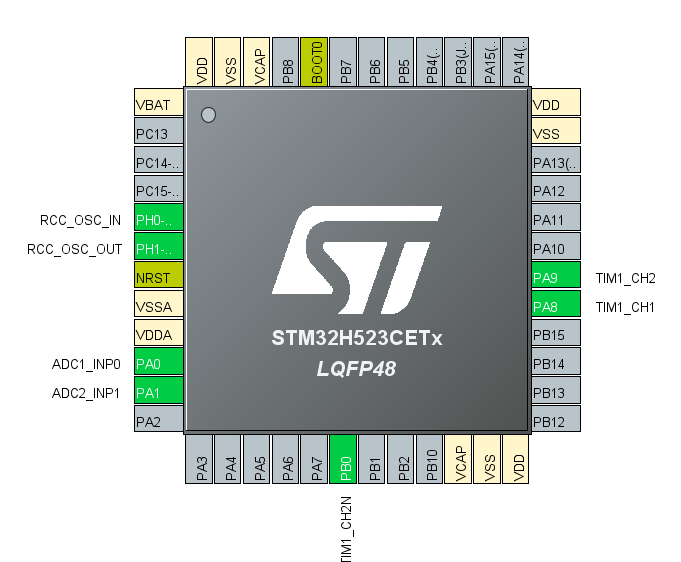
\includegraphics[width=0.7\linewidth]{src/IOC.png}
    \caption{Configuración de STM32F411}
    \label{fig:placeholder}
\end{figure}

\subsection{Driver de MOSFET IR2110}
La necesidad de un driver para MOSFET surge debido a la capacitancia parásita de la compuerta ($G$) de estos componentes. Para conmutar a frecuencias de cientos de kilohertz de forma limpia, se requiere inyectar y extraer corrientes instantáneas elevadas que las salidas GPIO del microcontrolador (limitadas a unos pocos miliamperios a 3.3V) no pueden suministrar.

Se utiliza el circuito integrado \textbf{IR2110}, un driver de compuerta de alta velocidad capaz de manejar de manera independiente canales flotantes superiores (High-Side) e inferiores (Low-Side). El canal superior implementa un circuito de \textit{bootstrap} (diodo rápido D1 y capacitor flotante) para elevar la tensión de compuerta del MOSFET superior por encima de la línea de potencia de 24V, garantizando su correcta saturación.

\subsection{Circuito de Acoplo e Inyección de Offset}
Debido a que el ADC de la Blackpill solo puede leer tensiones en un rango unipolar positivo de $0$\,V a $3.3$\,V, una señal de audio convencional (corriente alterna con semiciclos negativos) dañaría el microcontrolador o sufriría un recorte severo. 

Para solucionar esto, se implementa una red de acoplo que consta de:
\begin{itemize}
    \item Un \textbf{capacitor de acoplo de entrada} ($C_{in}$) que bloquea cualquier componente de corriente continua (DC) proveniente de la fuente de audio analógica.
    \item Un \textbf{divisor de tensión} resistivo ($R_x = 10$\,k$\Omega$ y $R_x = 10$\,k$\Omega$) conectado a 3.3V y GND que inyecta un desfase o nivel de continua fijo (\textit{offset}), posicionando el punto de reposo del audio exactamente en la mitad del rango dinámico del ADC ($\approx 1.65$\,V). 
\end{itemize}

\subsection{Filtro de Demodulación LC Pasas Bajas}
La señal a la salida del puente inversor de potencia es una onda cuadrada de gran amplitud modulada en PWM. Para recuperar la información de audio analógica original y enviarla a la bocina, se requiere remover la portadora de alta frecuencia de conmutación.

Se implementa un \textbf{filtro LC pasas bajas de segundo orden}. La frecuencia de corte del filtro ($f_c$) se diseña para estar ligeramente por encima del rango audible ($\approx 22$\,kHz). De este modo, el filtro actúa como un integrador, extrayendo el valor promedio instantáneo de la señal PWM y entregando una señal senoidal pura a la carga del altavoz de 8\,$\Omega$.

%----------------------------------------------------------------------
\section{Implementación y Cálculos Circuitales}\label{sec:implementacion}

\subsection{Etapa de Potencia y Filtrado LC}
La etapa de potencia consiste en una configuración de conmutadores basados en MOSFETs de potencia \textbf{IRF740} configurados en una topología de medio puente o puente H completo. 

El filtro pasas bajas se calcula considerando una impedancia nominal del altavoz de $R_L = 8\,\Omega$ y una frecuencia de corte deseada de $f_c \approx 22$\,kHz. La fórmula para la frecuencia de corte de un filtro LC es:
\begin{equation}
f_c = \frac{1}{2\pi \sqrt{L C}}
\end{equation}
Con el fin de obtener una frecuencia aproximada definimos el valor del inductor en 220\,$\mu$H y el capacitor en 470\,nF, lo que nos da una frecuencia de corte de aproximadamente 20\,kHz, ideal para nuestro diseño.
Sustituyendo los valores de diseño ($R_L = 8\,\Omega$, $f_c = 22$\,kHz, $L = 220\,\mu$H) en la fórmula, se obtiene el valor del capacitor necesario para lograr la frecuencia de corte deseada:
$$
C = \frac{1}{(2\pi f_c)^2 L} \approx \frac{1}{(2\pi \cdot 22000)^2 \cdot 220 \times 10^{-6}} \approx 470\,\text{nF}

$$

La implementación del circuito puede verse en la siguiente figura

\begin{figure}[!h]
    \centering
    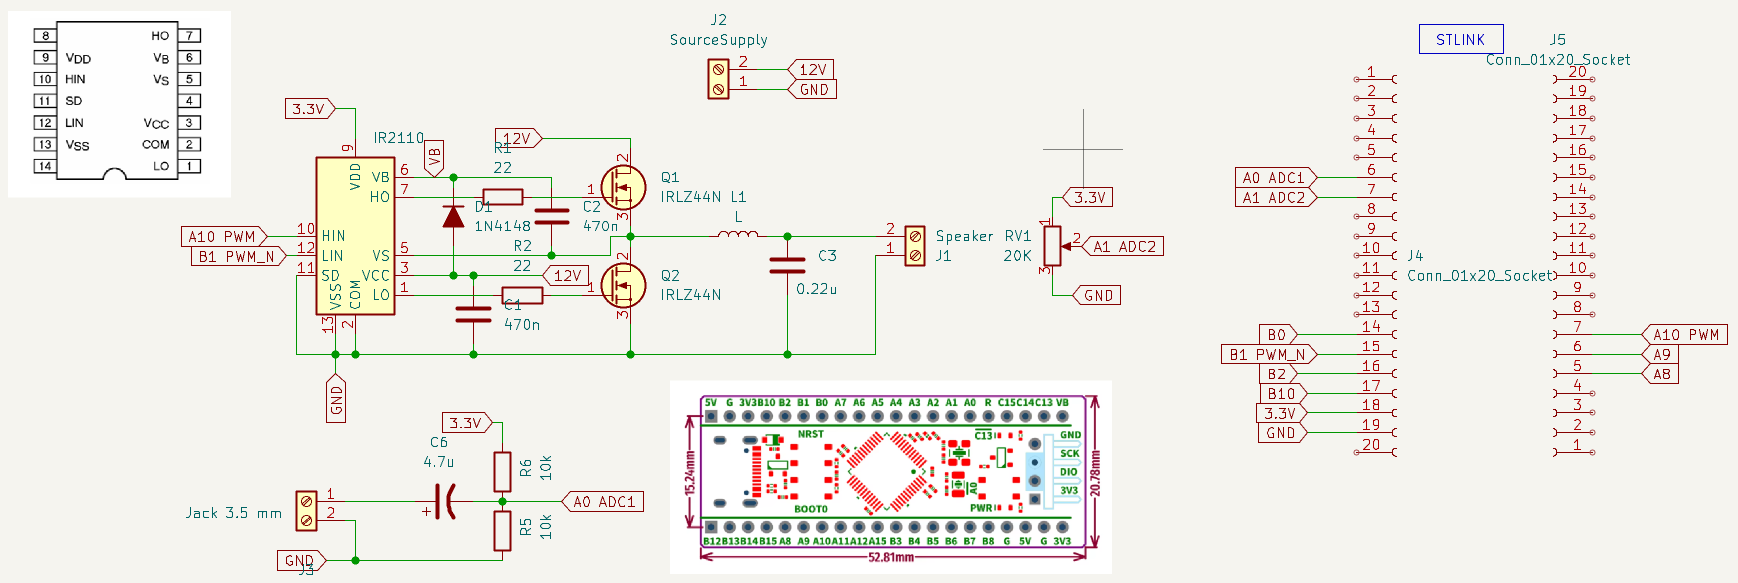
\includegraphics[width=\linewidth]{src/Esquematico.png}
    \caption{Esquemático}
    \label{fig:placeholder}
\end{figure}
\subsection{Regulación de Voltaje de Control}
El sistema requiere múltiples líneas de alimentación para las diferentes etapas lógicas y analógicas, derivadas de una fuente principal de 24V:
\begin{itemize}
    \item \textbf{+24V:} Línea de potencia principal para la conmutación de los MOSFETs de salida.
    \item \textbf{+15V:} Requerido por el driver IR2110 para proporcionar el voltaje de disparo suficiente a la compuerta de los MOSFETs (VCC y VB).
    \item \textbf{+3.3V:} Alimentación para la tarjeta STM32F411 Blackpill y la red de offset del ADC.
\end{itemize}
Para ello, se implementó un módulo regulador multietapa que reduce los 24V de entrada de manera eficiente a +15V y +3.3V usando reguladores integrados monolíticos protegidos con capacitores de desacoplo de $1\,\mu$F para filtrar ruidos de conmutación de alta frecuencia en las líneas de control.

%----------------------------------------------------------------------
\section{Fallas Típicas y Solución de Problemas}\label{sec:fallas}

Durante la puesta en marcha del amplificador Clase D se identificaron fallas críticas que fueron mitigadas mediante optimizaciones de diseño:

\subsection*{1. Conducción simultánea (Shoot-Through) en el Puente de Transistores}
El problema más severo en amplificadores Clase D es cuando el MOSFET superior e inferior conducen al mismo tiempo, creando un corto directo en la línea de 24V. Esto destruye instantáneamente los transistores. 
\begin{itemize}
    \item \textbf{Causa:} Retardos en el apagado de las compuertas de los MOSFETs.
    \item \textbf{Solución:} Configurar por software el bloque de \textit{Dead-Time Insertion} en los temporizadores avanzados de la Blackpill, asegurando un retraso mínimo de unos cientos de nanosegundos entre el apagado de un canal y el encendido del otro.
\end{itemize}


\newpage
\subsection*{3. Implementación en placa}
Una vez realizado las pruebas en la protoboard llegó la hora de pasarlo a placa, nuestra primer idea fue pasarlo a placa perforada, esto nos resulto algo complicado dado que la placa perforada era estilo protoboard y como no teníamos un buen esquemático en protoboard terminó provocando varias confusiones en cuanto a la orientación de los componentes
\begin{figure}[!h]
    \centering
    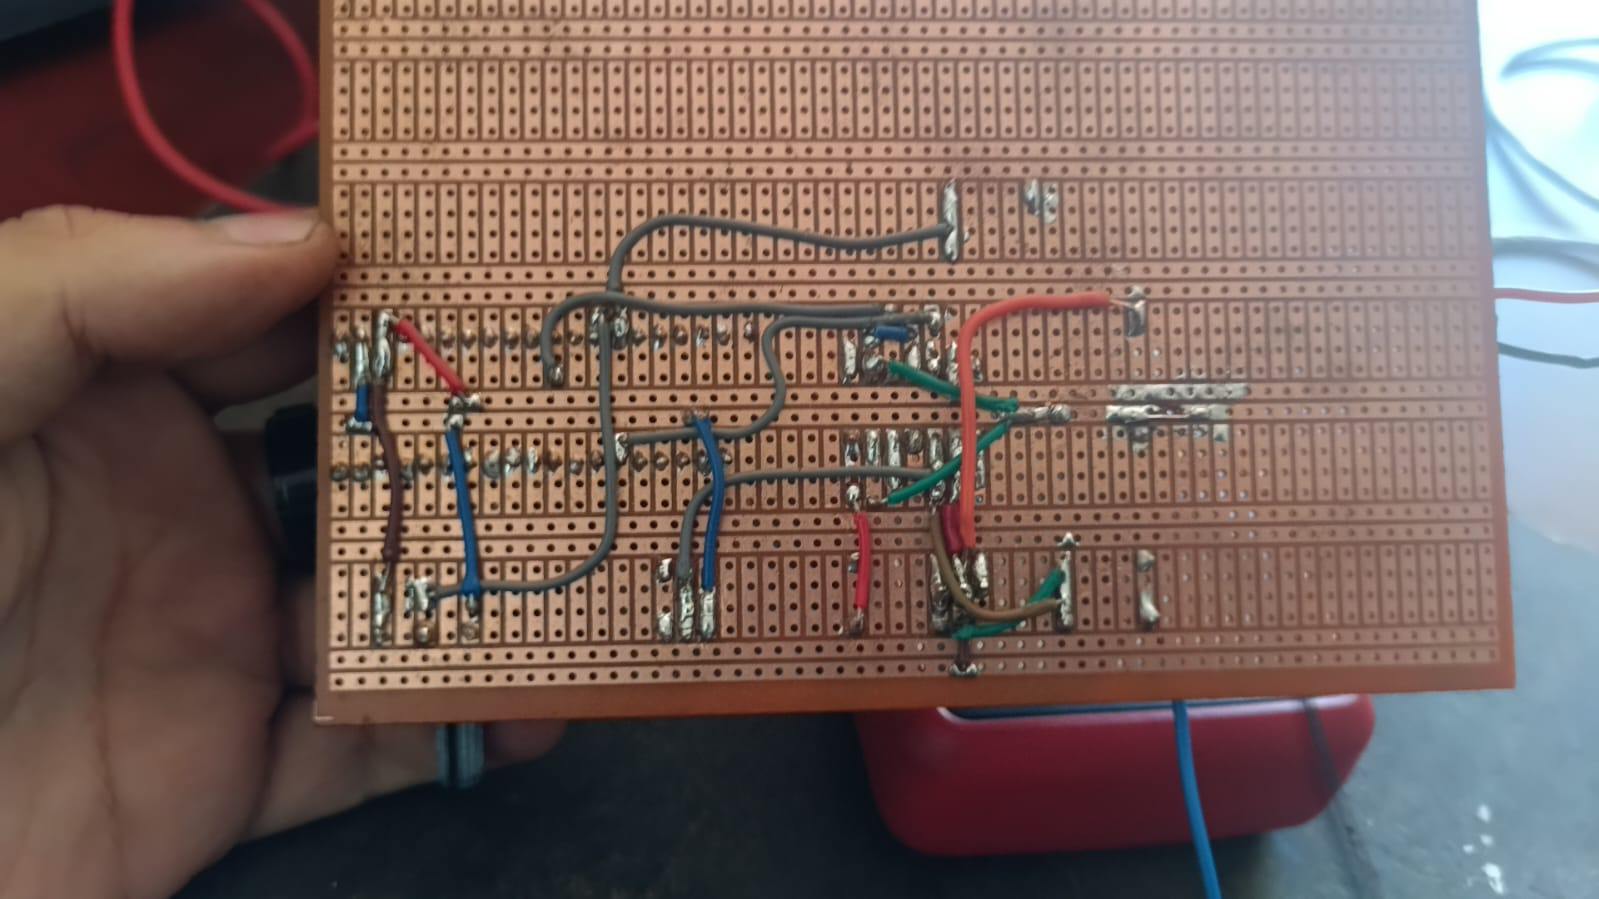
\includegraphics[width=0.6\linewidth]{src/Placa Perforada.png}
    \caption{Placa Perforada}
    \label{fig:placeholder}
\end{figure}

Finalmente decidimos hacerlo en una placa fenollica con la impresión y el grabado, fue aquí donde sucedió otro error que fue el considerar las huellas \textit{footprints}, de lado incorrecto lo que llevó a una inversión de componentes, en este caso por cuestiones de tiempo optamos por conectar el integrado IR2110 del lado correcto tal y como se muestra en la siguiente imagen.

\begin{figure}[!h]
    \centering
    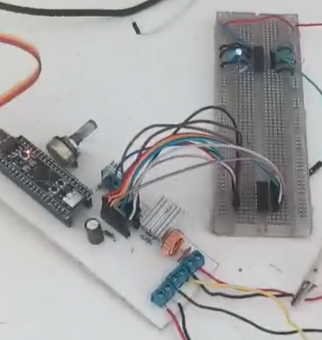
\includegraphics[width=0.5\linewidth,angle = 90]{src/PCB.png}
    \caption{Placa PCB con extensión para el IR2110}
    \label{fig:placeholder}
\end{figure}

Pese a las complicaciones se logró un amplificador clase D de forma exitosa, con una eficiencia energética superior al 90\% y una respuesta en frecuencia plana en el rango audible, demostrando la viabilidad de esta arquitectura para aplicaciones de audio de potencia controlada digitalmente. Además se estuvo probando con diferentes altavoces y diferentes aplicaciones de música como lo fue Youtube, Spotify y Tidal, viendo una mejora significativa en la calidad de audio.
\newpage
%----------------------------------------------------------------------
\section{Conclusiones}\label{sec:conclusiones}

El desarrollo de este amplificador de audio Clase D acoplado a la tarjeta STM32F411 Blackpill permitió concretar con éxito los siguientes puntos:
\begin{enumerate}
    \item \textbf{Eficiencia Tecnológica:} Se comprobó experimentalmente la superioridad en eficiencia de los sistemas conmutados frente a las configuraciones lineales clásicas analizadas previamente en el curso, reduciendo drásticamente las pérdidas térmicas en los transistores de salida.
    \item \textbf{Robustez del Control Digital:} El microcontrolador Blackpill demostró una capacidad de cómputo óptima para realizar los ciclos de muestreo mediante ADC y la subsecuente generación de señales PWM complementarias de alta frecuencia con tiempos muertos precisos, evitando fallas por cortocircuito.
    \item \textbf{Integración Analógica-Digital:} El correcto diseño de periféricos externos —como la inyección de offset para el ADC, la respuesta bootstrap del driver IR2110 y el filtrado pasivo LC final— evidenció que el éxito de un sistema embebido de potencia radica en la perfecta armonía entre el software de control y el hardware analógico de soporte.
\end{enumerate}

\section{Retroalimentación Personal del Curso}\label{sec:retroalimentacion}
\begin{itemize}
    \item \textbf{Contreras R. Orlando:} 
    La transición hacia el análisis de sistemas conmutados y procesamiento digital de potencia representó un reto excelente. Integrar conocimientos de programación en C para la Blackpill junto con el comportamiento físico de componentes como el driver IR2110 nos brindó una perspectiva real y sumamente demandada en el diseño de sistemas electrónicos modernos.
    
    \item \textbf{Lara H. Kevin:} 
    El proyecto me permitió afianzar el diseño práctico de hardware de audio. Considero que la materia aporta las bases ideales, y tener la libertad de desarrollar un amplificador de alta eficiencia nos motivó a profundizar en el filtrado de ruido y optimización de layouts para alta frecuencia.
    
    \item \textbf{García B. Iker:} 
    Aprecié enormemente el enfoque multidisciplinario de esta etapa. Solucionar problemas en tiempo real como los tiempos muertos en software para evitar cortos físicos en los MOSFETs te hace entender el impacto crítico de cada línea de código en los circuitos físicos.
\end{itemize}

\end{document}
